\section{Materials and methods}

The analysis uses two comparisons to examine the thermal information in a length-calibrated field. The first retains the B-fitted effective source-power fraction when assessing width, depth and the other operating conditions. The second changes the above-table conductivity and sensible specific heat at B, with B's source power and the phase law retained. Rear solidus and liquidus positions distinguish displacement of the cooling interval from a change in its spatial extent; scan speed then converts that extent to a passage time for stationary material.

\subsection{Benchmark observations and comparison design}
\label{sec:benchmark-design}
The benchmark comprises constant-speed single-track laser scans on bare IN625 plate made on the Additive Manufacturing Metrology Testbed (AMMT)~\cite{lane2020}, under the three public conditions in Table~\ref{tab:conditions}. Conditions B and C share the same applied power and differ in scan speed; condition A combines a lower power with a lower speed. The effective source-power fraction $\eta$ scales the power supplied to the conduction model to $\eta P$. It is fitted to B length and retained in the comparisons described below. The measured beam diameter is $D_{4\sigma}=170$~\um{}~\cite{lane2020}. For the assumed circular Gaussian, $D_{4\sigma}=2w$, giving $w=85$~\um. This reconstruction matches the measured second-moment diameter with circular symmetry; the published beam measurement retains a two-dimensional intensity map.

\begin{table}[htbp]
\centering
\caption{AMMT operating conditions and model energy scales. The effective source-power fraction $\eta\approx0.28905$ is fitted to B thermographic length only. $E_\ell=\eta P/v$ and $w/v$ are model input scales.}
\label{tab:conditions}
\begin{tabular}{lrrrr}
\toprule
Condition & $P$ (W) & $v$ (m/s) & $E_\ell$ (J/m) & $w/v$ (\us)\\
\midrule
A & 137.9 & 0.4 & 99.65 & 212.50\\
B & 179.2 & 0.8 & 64.75 & 106.25\\
C & 179.2 & 1.2 & 43.17 & 70.83\\
\bottomrule
\end{tabular}
\end{table}

Length targets are the AMMT-20~\us{} thermographic class means reported by Lane et al.~\cite{lane2020}. Their A/B/C populations contain 19/10/7 video frames, respectively. Width and depth are compared with the NIST challenge Table~2 metallographic means for the AMMT-100~\us{} specimen: three tracks each for A and B, and four for C~\cite{nist2018}. Lane's later cross-section compilation combines the 100 and 20~\us{} microscopy classes~\cite{lane2020}. Length and cross-sectional dimensions consequently enter as condition-level measurements from separate sampling populations, rather than three jointly observed dimensions of one pool.

The published geometric targets were consulted during model development, so the post-calibration comparisons are retrospective and nonblind. Only condition B length enters the calibration objective; B width/depth and all A/C dimensions are assessed with the resulting source-power fraction. Expanded uncertainties $U$ with coverage factor $k=2$ are taken from Lane's uncertainty budgets~\cite{lane2020}. For width and depth, these scales belong to the combined-class microscopy analysis, whereas the target means belong to the NIST 100~\us{} classes. Each signed difference $\delta=Q_{\rm model}-Q_{\rm measurement}$ is also reported as $\delta/U$, a descriptive normalization by that published measurement scale. The denominator does not include model, input or calibration uncertainty, and the width/depth ratios do not constitute a formal uncertainty test of the 100~\us{} target means.

\subsection{Moving-frame enthalpy model and high-temperature properties}
The conduction model accounts for sensible and latent energy through a conservative enthalpy formulation~\cite{vanelsen2007}. This permits conductivity and sensible specific heat to be changed separately while preserving one phase law. The laboratory-frame balance is
\begin{equation}
 \frac{\partial H}{\partial t}=\nabla\cdot[k(T)\nabla T],\qquad
 H(T)=\rho\left[\int_{T_0}^{T}c_p(s)\,\mathrm ds+\mathcal L f(T)\right].
 \label{eq:enthalpy}
\end{equation}
The density $\rho=8440$~\si{\kilogram\per\cubic\metre} follows the IN625 supplier bulletin; its listed melting range supplies the adopted thresholds $T_s=1290$~$^\circ$C and $T_l=1350$~$^\circ$C~\cite{specialmetals625}. The latent heat $\mathcal L=280000$~\si{\joule\per\kilogram} follows the earlier AMMT model~\cite{kollmannsberger2019}; the reference temperature is set to $T_0=25$~$^\circ$C. A linear liquid-fraction approximation distributes this latent heat over the adopted interval. A linear phase-fraction relation is also used in a continuum IN625 model~\cite{dynamic2024}, although that study selects a different freezing interval. Here the liquid fraction is
\begin{equation}
 f(T)=\begin{cases}
 0,&T<T_s,\\
 (T-T_s)/(T_l-T_s),&T_s\leq T<T_l,\\
 1,&T\geq T_l.
 \end{cases}
\end{equation}
Sensible specific heat and conductivity are linearly interpolated between the input knots in Table~\ref{tab:properties}. The conductivity table contains 15 points and ends at 982~$^\circ$C; the 12-point specific-heat table ends at 1093~$^\circ$C. The supplier labels specific heats as calculated and conductivity as measured, with the conductivity measurements made at Battelle on material annealed at 2100~$^\circ$F for 1~h~\cite{specialmetals625}. These are typical alloy data rather than benchmark-coupon measurements. Within the adopted phase interval, differentiating Eq.~\eqref{eq:enthalpy} gives $c_{p,\mathrm{eff}}=c_p+\mathcal L/(T_l-T_s)$, with a latent contribution of 4666.67~\si{\joule\per\kilogram\per\kelvin}. Retaining this contribution in every case distinguishes a change in sensible specific heat from a change in latent heat.

Both tables end below the adopted solidus, so the solution through the melting interval requires an above-table property definition. The closest AMMT conduction study likewise identified high-temperature conductivity extrapolation as a modeling assumption that participates in calibration~\cite{kollmannsberger2019}. Figure~\ref{fig:properties} defines the two extrapolation rules examined here.

\begin{figure}[htbp]
\centering
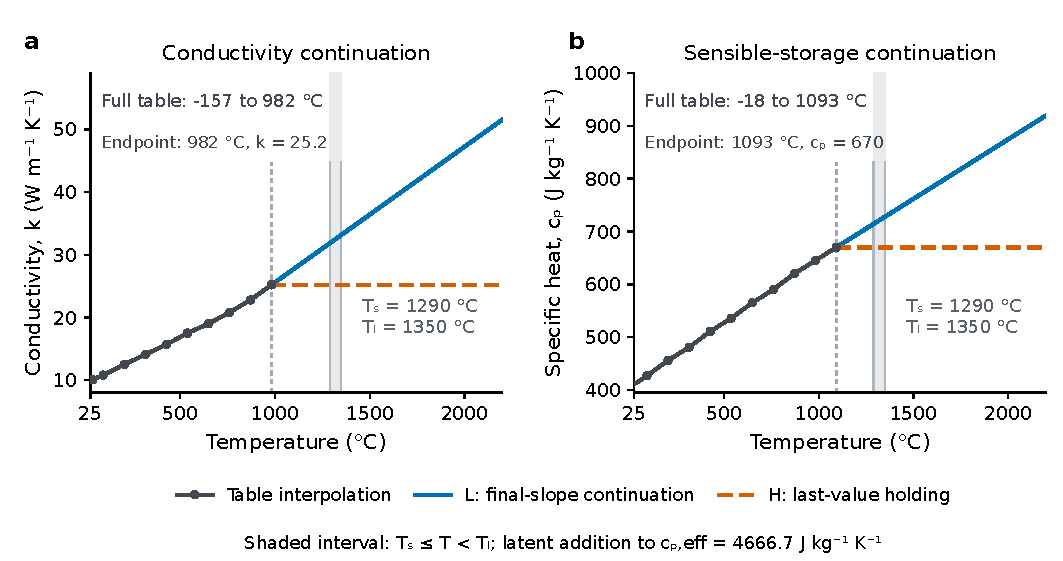
\includegraphics[width=\textwidth]{figures/ammt-property-continuations.pdf}
\caption{IN625 property inputs and extrapolation definitions. (a) Conductivity and (b) sensible specific heat use the knots in Table~\ref{tab:properties}, with common piecewise-linear interpolation below their respective endpoints. The final knots are 982~$^\circ$C and 25.2~\si{\watt\per\metre\per\kelvin} for $k$, and 1093~$^\circ$C and 670~\si{\joule\per\kilogram\per\kelvin} for $c_p$. L denotes final-secant linear extrapolation and H constant endpoint extrapolation, as defined in Eq.~\eqref{eq:property-extrapolation}. The displayed window is 25--2200~$^\circ$C; all 15 conductivity and 12 specific-heat source rows, including those below 25~$^\circ$C, are retained in the accompanying data and used in interpolation. Shading marks the adopted 1290--1350~$^\circ$C phase interval. The latent addition to effective specific heat within this interval is 4666.7~\si{\joule\per\kilogram\per\kelvin}, separate from sensible $c_p$. The supplier describes conductivity as measured and specific heat as calculated typical alloy data~\cite{specialmetals625}; the above-table functions are study-defined choices.}
\label{fig:properties}
\end{figure}

For either property $p\in\{k,c_p\}$, let $(T_{n-1},p_{n-1})$ and $(T_n,p_n)$ be its final two tabulated pairs. Above $T_n$, final-secant linear extrapolation (L) and constant endpoint extrapolation (H) are defined by
\begin{equation}
 p_{\rm L}(T)=p_n+\frac{p_n-p_{n-1}}{T_n-T_{n-1}}(T-T_n),\qquad
 p_{\rm H}(T)=p_n,\qquad T>T_n.
 \label{eq:property-extrapolation}
\end{equation}
Thus H uses $k=25.2$~\si{\watt\per\metre\per\kelvin} above 982~$^\circ$C and $c_p=670$~\si{\joule\per\kilogram\per\kelvin} above 1093~$^\circ$C; the appendix lists the final-secant slopes. Each change applies above its table endpoint, including the solid range between that endpoint and $T_s$. Conductivity changes are applied consistently to $k$, its primitive $K$ and the inverse used for surface-temperature recovery. Specific-heat changes are applied to $c_p$, the enthalpy $H$ and its inverse $T(H)$. The archived two-letter labels place conductivity first: LL uses linear extrapolation for both properties, HL and LH change one property, and HH changes both. These functions define numerical property scenarios rather than bounds on measured liquid properties.

Following the moving-source coordinate description~\cite{vanelsen2007}, let $\xi=x-vt$. For a quasi-steady field, $\partial_tH=-v\partial_\xi H$; defining $\bm u=(-v,0,0)$ therefore gives
\begin{equation}
 \nabla\cdot(\bm uH-k\nabla T)=0.
 \label{eq:frame}
\end{equation}
The term $\bm uH$ represents stationary material passing through the laser coordinate frame. No liquid momentum equation or melt convection is included. The assumptions also exclude evaporation and free-surface deformation.

The circular Gaussian surface input at $z=0$, normalized consistently with the $D_{4\sigma}$ convention~\cite{dynamic2024}, is
\begin{equation}
 q(\xi,y)=\frac{2\eta P}{\pi w^2}
 \exp\!\left[-\frac{2(\xi^2+y^2)}{w^2}\right].
 \label{eq:source}
\end{equation}
Its full-plane integral is $\eta P$, so fitting $\eta$ adjusts the total input power while retaining the source shape; it does not measure absorptivity independently of the adopted model. With outward normal $\bm n$, the top condition is $-k\nabla T\cdot\bm n=-q$, supplying inward heat. The appendix gives the discrete source integration. At positive $\xi$, incoming material has $H=0$; at negative $\xi$, diffusive gradient vanishes and enthalpy leaves advectively. The $y=0$ plane is symmetric. Outer transverse and bottom boundaries are adiabatic. Radiation and ambient convection are omitted from the solved balance.

\subsection{Geometry, rear phase boundaries and material passage}
\label{sec:geometry-passage}
The model solidus-crossing length $L$ is the distance between the front and rear crossings of the recovered surface symmetry-centerline temperature. These crossings are interpolated, must enclose the source, and must form one interval without domain truncation. Surface and symmetry-plane recovery precede threshold extraction; the appendix gives their numerical definitions. Retaining both positions allows a change in total length to be assigned to motion at the front or rear.

Fusion-zone width and depth are extracted from the source-connected component of
\begin{equation}
 T_{\max}(y,z)=\max_\xi T(\xi,y,z)\geq T_s.
 \label{eq:fusion}
\end{equation}
Each $\xi$ slice is reconstructed at the surface and symmetry plane, bilinearly interpolated onto observation coordinates, and then maximized over passage. This order defines the maximum-temperature fusion envelope; maximizing nodal temperatures before interpolation gives a different envelope. Width is twice the positive-$y$ extent and depth is the negative of the lowest $z$. The observation pitch controls sampling of the reconstructed geometry. Figures label the model surface-length proxy $L_s$ and fusion-envelope extents $W_f$ and $D_f$; these correspond to $L$, $W$ and $D$ in the text. A separate surface-sample maximum is taken over the recovered top-surface temperatures at axial and positive-$y$ cell-center coordinates, before the $y=0$ extension. It therefore has a different sampling definition from the symmetry-centerline field used for the crossings.

Lane's thermographic length locates the rear freezing feature from a radiance-profile second-derivative minimum, then finds the front at the assumed freezing temperature after emittance-based conversion~\cite{lane2020}. This measured length includes the effects of emittance, exposure and viewing geometry. The model instead uses two solidus crossings of a recovered temperature field. Its fitted $\eta$ consequently belongs to the combination of source, material law and boundary definition used here. Fusion-envelope width and depth are compared with the metallographic dimensions defined in Section~\ref{sec:benchmark-design}.

Let $\xi_s^-$ and $\xi_l^-$ denote the rear centerline solidus and liquidus crossings. Their positions locate the adopted freezing interval relative to the source; their separation gives its spatial extent. Define this rear solidus--liquidus separation, passage time and interval-mean cooling-rate magnitude as
\begin{equation}
 \ell_m=\xi_l^- -\xi_s^-,\qquad
 \tau_m=\frac{\ell_m}{v},\qquad
 \overline{\dot T}=\frac{T_l-T_s}{\tau_m}.
 \label{eq:passage}
\end{equation}
At a fixed laboratory point, $\mathrm d\xi/\mathrm dt=-v$, so the material traverses the rear interval in $\ell_m/v$. The same spatial separation can therefore correspond to different passage times at different scan speeds. Constant-speed space-to-time mapping is also used in the AMMT measurements~\cite{lane2020}, but their cooling estimate covers a below-solidus interval, while Eq.~\eqref{eq:passage} uses 1350--1290~$^\circ$C. Lane et al. present their cooling rates as exemplar data rather than model-calibration references~\cite{lane2020}. Here, separation, time and interval-mean cooling rate are derived from the same modeled field; the passage follows stationary material rather than a moving liquid parcel.

\subsection{Length calibration and property comparisons at retained source power}
With LL properties, fitting $L_B(\eta)=359$~\um{} gives $\eta\approx0.28905$, with a signed length residual of +0.158~\um. Conditions A and C retain this value, beam, phase law and property extrapolations. The appendix gives the safeguarded scalar calibration algorithm, trial values and local sensitivity. This length fit sets the effective source-power fraction across A, B and C, and fixes the source power within the four B property cases.

The four B cases share power, speed, beam, density, phase thresholds, latent heat, mesh, observation operators and the source-power fraction fitted with LL properties. Only the above-table $k$ and $c_p$ definitions change, including their corresponding primitives and recovery operations. The first letter denotes conductivity and the second sensible specific heat. Sharing B=LL between the three-condition geometry comparison and the four-case property comparison gives six production solutions. Retaining the LL-fitted factor makes the other B cases responses at common source power, rather than separate length fits.

For any output $Q$, define the baseline-anchored finite effects
\begin{align}
 \delta_k&=Q_{\HL}-Q_{\LL}, &
 \delta_{c_p}&=Q_{\LH}-Q_{\LL},\\
 I_{k,c_p}&=Q_{\HH}-Q_{\HL}-Q_{\LH}+Q_{\LL}, &
 \Delta_{\rm joint}&=Q_{\HH}-Q_{\LL}=\delta_k+\delta_{c_p}+I_{k,c_p}.
 \label{eq:contrast}
\end{align}
At constant-extrapolated $c_p$, the conductivity effect is $Q_{\HH}-Q_{\LH}=\delta_k+I_{k,c_p}$; at constant-extrapolated $k$, the specific-heat effect is $Q_{\HH}-Q_{\HL}=\delta_{c_p}+I_{k,c_p}$. Reporting these conditional effects establishes whether each response direction persists at both levels of the other property. The interaction records the departure of the joint change from the sum of the two LL-anchored changes. All effects are deterministic finite differences between specified functions within this conduction model.

An axial-face P\'eclet diagnostic compares coordinate enthalpy transport with diffusion in the phase interval. A discrete rear hot-region budget measures net outward diffusive power. Each branch defines its temperature-selected region separately, allowing the diagnostic population and region boundary to follow the solved field. These budgets complement the matched-coordinate phase thresholds; their definitions are given in the appendix.

\subsection{Numerical solution and verification}
The conservative finite-volume solution uses near-source cell widths of $4\times3\times1$~\um. Gaussian power is integrated over each top-face rectangle and supplied to its adjacent control volume; surface-temperature recovery uses the corresponding conductivity primitive. Conductivity and enthalpy relations are updated with the nonlinear solution, so each extrapolation case changes the material functions consistently. The graded-domain geometry, scaled enthalpy discretization and recovery equations are specified in the appendix. Convergence is checked using both the sum of absolute cell residuals and the signed global energy balance, followed by a full frozen-coefficient correction.

A separate constant-property moving-Gaussian problem checks source integration, frame transport and geometric extraction against a semi-infinite analytical reference. This verification isolates numerical implementation from assessment against physical measurements~\cite{oberkampf2002}. Its reference $L/W/D$ is $407.535/153.293/34.836$~\um; finite-volume differences are +0.139\%, +0.190\% and $-0.499$\%, respectively. The benchmark uses constant properties and omits phase change, making its accuracy assessment specific to that verification problem.

At the calibrated $\eta$, reducing the near-source axial spacing from 4 to 2~\um\ changes B length, width and depth by +0.361, $-0.009$ and +0.041~\um, and C by +0.199, $-0.029$ and +0.045~\um. A/B domain enlargement changes these quantities by less than $3\times10^{-6}$~\um. These measured sensitivities support the interpretation of the larger geometric responses, but do not give a full three-dimensional error bound for every extrapolation case. Submicrometre interactions are consequently reported descriptively.

An earlier transient B comparison at a different calibration stage provides approximate local steady consistency. Fixed-field blackbody estimates put B-case top losses at 0.099--0.180\% of absorbed power; feedback from these losses is not solved. These checks have distinct roles from the constant-property verification and the calibrated-mesh comparisons.

All six solutions satisfy the stated energy-balance and nonlinear-correction criteria and give bounded phase fractions and nontruncated extracted geometry. The appendix reports the acceptance thresholds and final residuals.

\section{Results}
The post-calibration geometry comparison identifies which aspects of the fusion shape remain discrepant after fitting length. The B property comparison then resolves whether its length response arises mainly from motion of the rear phase boundaries or from a change in their separation. The fixed-power B--C comparison finally relates the spatial separation to material passage time at different scan speeds.

\subsection{Geometry discrepancy after length calibration}
Fitting the source-power fraction to B thermographic length gives a model length of 359.16~\um{}, but leaves a wider and shallower fusion envelope than the B metallographic means (Table~\ref{tab:geometry} and Fig.~\ref{fig:comparison}). Model width exceeds the NIST 100~\us{} class mean by 19.54~\um{}, and depth falls below it by 4.88~\um. Normalizing these differences by Lane's published combined-class microscopy uncertainty scales gives +3.10 and $-1.23$, respectively. The fitted axial extent therefore does not reproduce the transverse fusion shape in this model.

\begin{table}[htbp]
\centering
\caption{Model geometry and AMMT measurement means in \um. Length means are from Lane's 20~\us{} thermography classes; width/depth means are from the current NIST 100~\us{} metallography classes. $U$ is Lane's separately sourced expanded measurement uncertainty ($k=2$); width/depth $U$ comes from its combined-class microscopy analysis. B length is fitted. $\delta/U$ is a descriptive difference normalized by that published scale, without combined model uncertainty.}
\label{tab:geometry}
\small
\begin{tabular}{llrrrr}
\toprule
Condition & Quantity & Model & Measured mean & $U$ & $\delta/U$\\
\midrule
A & $L$ & 309.89 & 300 & 11.91 & +0.83\\
  & $W$ & 153.36 & 147.9 & 6.42 & +0.85\\
  & $D$ & 40.47 & 42.5 & 4.49 & $-0.45$\\
B & $L$ (fitted) & 359.16 & 359 & 21.26 & +0.01\\
  & $W$ & 143.04 & 123.5 & 6.30 & +3.10\\
  & $D$ & 31.12 & 36 & 3.97 & $-1.23$\\
C & $L$ & 320.63 & 370 & 32.57 & $-1.52$\\
  & $W$ & 129.05 & 106 & 4.48 & +5.14\\
  & $D$ & 22.04 & 29.6 & 3.26 & $-2.32$\\
\bottomrule
\end{tabular}
\end{table}

\begin{figure}[htbp]
\centering
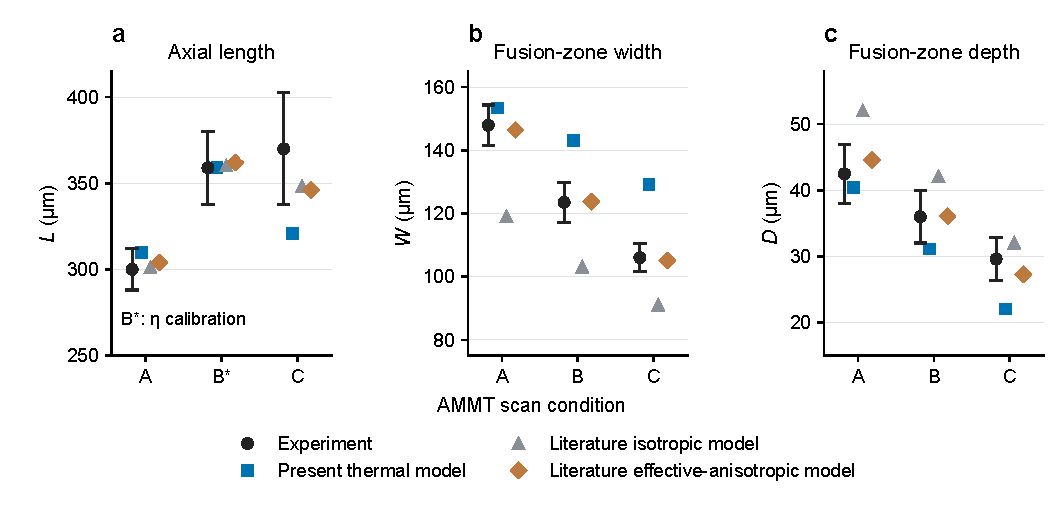
\includegraphics[width=\textwidth]{figures/ammt-application-experiment.pdf}
\caption{Geometry comparison with Lane's 20~\us{} thermographic length means, NIST's 100~\us{} metallographic width/depth means, and the published isotropic and effective-anisotropic calculations of Kollmannsberger et al.~\cite{kollmannsberger2019}. Experimental bars show separately sourced Lane $U(k=2)$ scales; width/depth centers use current NIST means. B length is calibrated in the present model. Published-model points provide context under different beam representations, material/phase laws, calibration targets and observation definitions; their differences from the present results are not a single-factor comparison.}
\label{fig:comparison}
\end{figure}

Condition A deviations are smaller than their respective published measurement-uncertainty scales. In C, the model is 49.37~\um{} shorter than the thermographic mean, 23.05~\um{} wider and 7.56~\um{} shallower than the NIST metallographic means. The modeled aspect ratios $W/D=3.79,4.60,5.85$ for A/B/C also show the widening relative to penetration, compared with ratios of the measured class means of 3.48,3.43,3.58 (Fig.~\ref{fig:trends}b). These measured ratios are formed from condition-level means, rather than paired with each thermographic length frame.

At fixed power from B to C, a 50\% speed increase reduces model input energy per unit length, $\eta P/v$, by one third. Model width decreases by 9.78\% and depth by 29.16\%; the NIST metallographic class-mean changes are 14.17\% and 17.78\% (Fig.~\ref{fig:trends}a). The modeled $W/D$ consequently increases by 27.36\% from B to C. The geometry discrepancy thus concerns both absolute dimensions and how transverse contraction compares with reduced penetration as speed rises. Condition A also changes power, so the B--C pair provides the fixed-power speed comparison.

The thermographic class mean increases in length by 11~\um\ from B to C, whereas model length decreases by 38.53~\um. The two reported expanded-uncertainty scales give a zero-correlation quadrature of 38.89~\um, larger than the change between measured means. This descriptive scale comparison limits interpretation of the sign of the measured B--C trend; the C residual in Table~\ref{tab:geometry} compares C with its own mean. The observed axial-refinement changes below 0.37~\um\ are much smaller than the main B/C residuals, so the retained refinement evidence does not remove the principal shape discrepancy.

\begin{figure}[htbp]
\centering
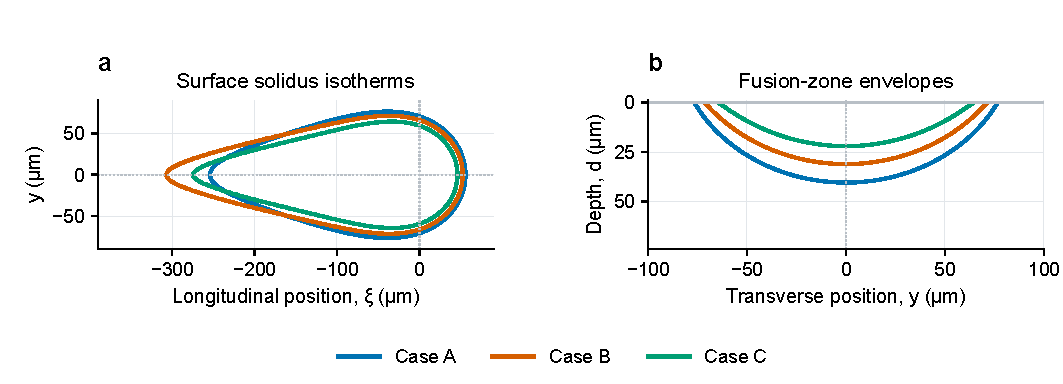
\includegraphics[width=\textwidth]{figures/ammt-research-operating-cases.pdf}
\caption{Model geometry for A, B and C. (a) Surface solidus contours in laser-frame coordinates. (b) Reconstructed maximum-temperature fusion envelopes in transverse/depth coordinates. Fusion envelopes use slice reconstruction and interpolation before passage maximization. Both panels display calculated thermal geometry and use the fixed calibrated source factor.}
\label{fig:fields}
\end{figure}

The contours in Fig.~\ref{fig:fields} show the greater fractional reduction in penetration than in width for the fixed-power B--C comparison. The surface solidus contour supplies the model length, while the transverse envelope records the maximum melted extent during material passage. Since a length fit leaves this shape discrepancy, the B property comparison examines how the constitutive definitions change the fitted field's rear boundaries, with the calibrated source-power fraction retained.

\subsection{Property effects on rear-boundary position and separation}
\label{sec:property-results}
At the B-fitted source power, the two property changes produce opposing length responses (Table~\ref{tab:factorial}). Replacing final-secant linear extrapolation of conductivity by constant endpoint extrapolation increases length from 359.16 to 402.37~\um\ when $c_p$ remains linear (LL to HL). Changing only $c_p$ to constant endpoint extrapolation decreases length to 352.99~\um\ (LL to LH). Changing both yields 393.44~\um\ (HH), so
\begin{equation}
 \Delta L_{\rm joint}=43.21-6.17-2.76=34.28~\um.
\end{equation}
The specific-heat response and interaction offset part of the conductivity-induced increase. These response directions persist at the other factor level: constant extrapolation of conductivity increases length by 40.45~\um{} at constant-extrapolated $c_p$, and constant extrapolation of $c_p$ decreases length by 8.93~\um{} at constant-extrapolated $k$. Thus the direction of each length response is consistent across the two tested levels of the other property.

\begin{table}[htbp]
\centering
\caption{Two-factor property comparison at B and the LL-fitted source-power fraction. The first letter labels $k$, the second $c_p$; L denotes final-secant linear extrapolation and H constant endpoint extrapolation above the respective table endpoints. All cases retain the same source power and phase law. Rounded geometry and finite effects are in \um. Small transverse effects lack branch-specific refinement evidence.}
\label{tab:factorial}
\begin{tabular}{lrrr}
\toprule
Corner or contrast & $L$ & $W$ & $D$\\
\midrule
LL & 359.16 & 143.04 & 31.12\\
HL & 402.37 & 143.15 & 30.09\\
LH & 352.99 & 143.72 & 31.61\\
HH & 393.44 & 143.79 & 30.80\\
\midrule
$\delta_k$ & +43.21 & +0.11 & $-1.03$\\
$\delta_{c_p}$ & $-6.17$ & +0.68 & +0.49\\
$I_{k,c_p}$ & $-2.76$ & $-0.04$ & +0.21\\
$\Delta_{\rm joint}$ & +34.28 & +0.75 & $-0.32$\\
\bottomrule
\end{tabular}
\end{table}

The rear solidus and liquidus positions identify which part of the field produces these length changes (Fig.~\ref{fig:factorial}). From LL to HL, the rear crossings move by $-42.49$ and $-43.50$~\um{}, respectively, while the front solidus moves by +0.73~\um. Rear solidus displacement accounts for 98.3\% of the conductivity-induced length increase, with the front contributing 1.7\%. Yet the rear solidus--liquidus separation changes by only $-1.01$~\um. From LL to LH, the rear crossings instead move towards the source by +6.22 and +6.53~\um, with a separation change of +0.31~\um. The large length response therefore arises predominantly from displacement of the pair of rear phase boundaries, rather than a comparable change in the distance between them.

The two prescribed changes perturb conductivity and total storage by different relative amounts. At 1320~$^\circ$C, changing L to H reduces conductivity from 32.51 to 25.20~\si{\watt\per\metre\per\kelvin}, or 22.48\%, and sensible specific heat from 721.13 to 670~\si{\joule\per\kilogram\per\kelvin}, or 7.09\%. With the fixed latent contribution included, effective specific heat decreases from 5387.79 to 5336.67~\si{\joule\per\kilogram\per\kelvin}, or 0.95\%, and enthalpy from the cold reference decreases by 0.66\%. Their geometric effect sizes consequently compare these specified input changes rather than equal-percentage perturbations of transport and total storage.

The auxiliary transport diagnostics also change from LL to HL. The median axial-face P\'eclet diagnostic rises from 4.44 to 5.77, while integrated outward diffusion from the rear hot region rises from 14.724 to 14.913~W. The latter increase accompanies the lower conductivity: the solved gradients and the temperature-selected region boundary both change. These values therefore describe each field's selected faces and region, rather than conductive power through one fixed integration boundary. The conductivity case also uses its corresponding material primitive in surface-temperature recovery.

The recovered positive-$y$ surface-sample maxima defined in Section~\ref{sec:geometry-passage} are approximately 2697, 3507, 2756 and 3721~$^\circ$C for LL, HL, LH and HH, respectively. Both cases with constant-extrapolated conductivity give higher sampled temperatures. These are maxima of the stated surface samples, not an independently resolved maximum temperature of the melt pool; they also differ in sampling from the recovered $y=0$ profile used for phase-boundary positions. Their physical interpretation must retain the evaporation, flow and surface-deformation omissions of the conduction balance.

The current-mesh depth response contains opposing contributions. Constant extrapolation of conductivity changes depth by $-1.03$~\um{} from LL; the specific-heat change contributes +0.49~\um\ and the interaction +0.21~\um, leaving a joint change of $-0.32$~\um. Conductivity effects remain negative at both specific-heat levels ($-1.03$ and $-0.82$~\um), while specific-heat effects remain positive at both conductivity levels (+0.49 and +0.71~\um). Every case retains the B width excess and depth deficit. The extrapolation choices thus move the rear boundaries substantially while retaining the principal fusion-shape discrepancy. The 34--43~\um\ length response exceeds the retained baseline axial sensitivity by a wide margin; the 0.04~\um\ width interaction remains an unresolved fine-scale comparison pending branch-specific refinement.

\begin{figure}[htbp]
\centering
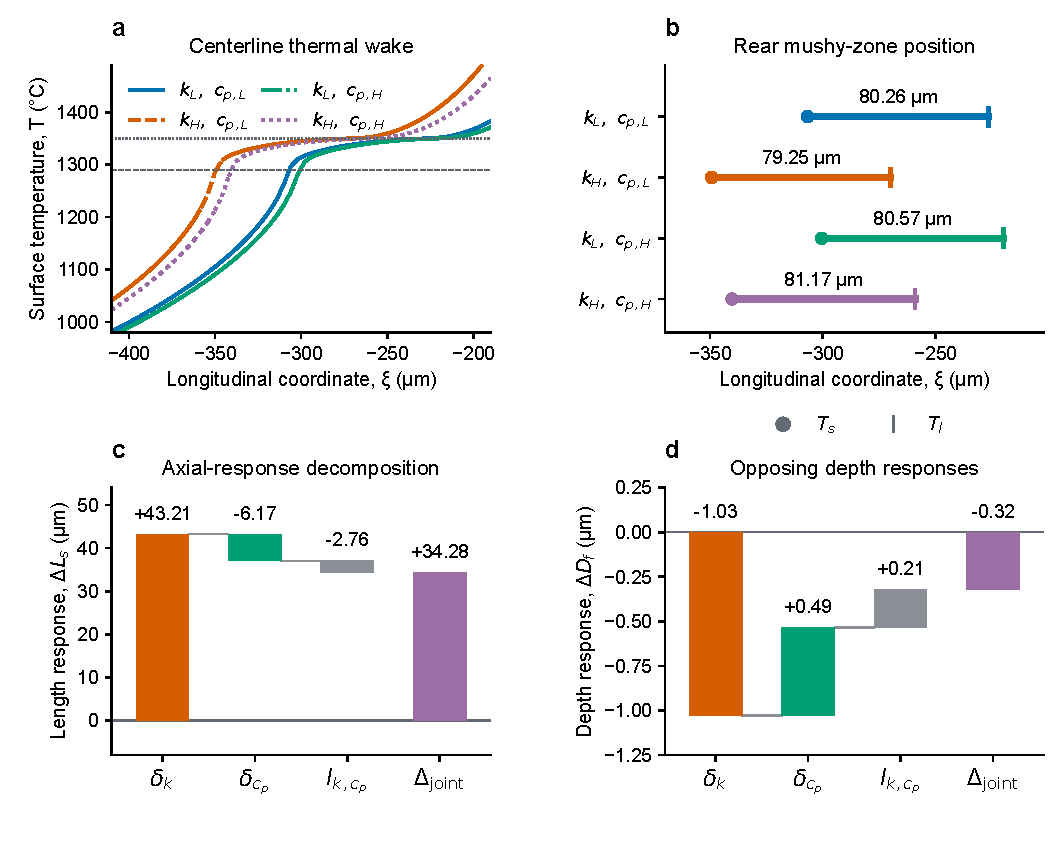
\includegraphics[width=\textwidth]{figures/ammt-research-constitutive-factorial.pdf}
\caption{Property comparison at B: rear centerline temperature profiles, solidus/liquidus positions and their separation, and LL-anchored geometry effects. All four cases retain the same phase thresholds, calibrated source-power fraction and mesh. Profiles are plotted from original field values with segment clipping to the displayed window. Factorial effects are deterministic finite differences between the defined extrapolation functions. Displacement of the rear boundary pair dominates the length response; the joint depth change contains opposing single-property contributions.}
\label{fig:factorial}
\end{figure}

Across the four cases, the rear solidus--liquidus separation lies between 79.25 and 81.17~\um{}, while total length ranges from 352.99 to 402.37~\um. The comparison therefore distinguishes a large response in the location of the rear freezing interval from a smaller response in its spatial extent. The fine ordering of those separations remains a current-mesh result.

\subsection{Scan speed and derived material passage time}
The fixed-power B--C comparison yields nearly equal rear solidus--liquidus separations at different scan speeds. On the present mesh, B and C give 80.26 and 80.79~\um{}, respectively, a difference of 0.53~\um{} (Fig.~\ref{fig:trends}c). Their corresponding passage times are 100.33 and 67.33~\us{} (Fig.~\ref{fig:trends}d). The C separation is 0.66\% larger, yet its passage time is 32.90\% shorter because speed increases from 0.8 to 1.2~m/s. The interval-mean cooling rate over 1350--1290~$^\circ$C consequently rises from 0.598 to 0.891~\si{\mega\kelvin\per\second}, an increase of 49.02\%. Condition A, which also changes power, gives a separation of 48.30~\um{}, a passage time of 120.74~\us{} and a cooling rate of 0.497~\si{\mega\kelvin\per\second}.

The 49.02\% B--C cooling-rate increase follows from the shorter passage through an almost unchanged spatial interval, using Eq.~\eqref{eq:passage}. It is a second expression of the same centerline separation and scan speed. The spatial interval alone cannot determine the time experienced by material.

\begin{figure}[htbp]
\centering
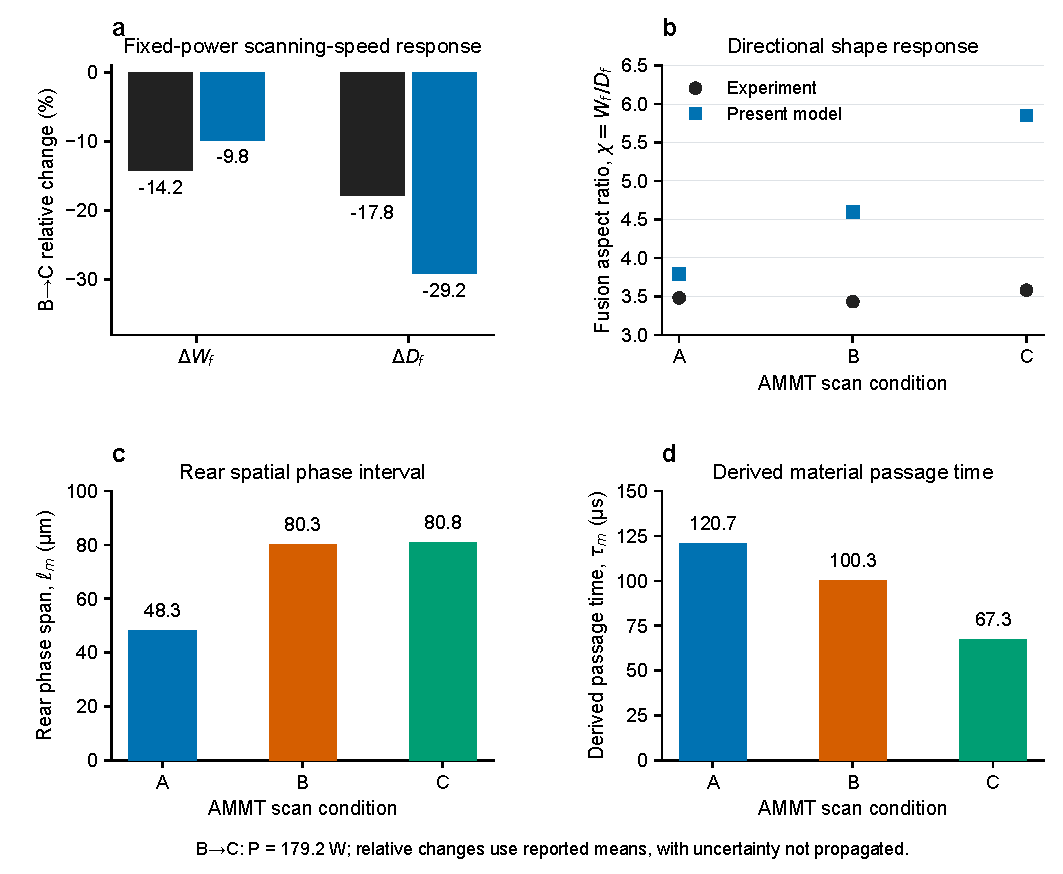
\includegraphics[width=\textwidth]{figures/ammt-research-condition-trends.pdf}
\caption{Operating-condition response. (a) B-to-C percentage changes in width and depth at fixed power, comparing the model with NIST 100~\us{} metallographic class means; uncertainty is not propagated. (b) Model and measured class-mean aspect ratios. (c) Model rear liquidus-to-solidus separations. (d) Derived material passage times. Separation and time are transformations of the same steady centerline field. The text reports the corresponding interval-mean cooling rates over 1350--1290~$^\circ$C.}
\label{fig:trends}
\end{figure}

The B--C pair consequently shows both contraction of the fusion envelope and faster passage through an almost unchanged rear freezing interval. The former response is assessed against metallographic dimensions; the latter characterizes stationary material crossing the calculated centerline field. It complements the rear-position comparison by distinguishing where cooling occurs from the distance and time over which the adopted freezing interval is traversed.
